\section{CHƯƠNG 7: DASHBOARD PHÂN TÍCH VIDEO}

% Chỉnh lại các hình minh họa: chụp rõ nét hơn + thay đổi vị trí đặt hình cho phù hợp (ht => H)
\subsection{Giới thiệu}

Dashboard này giúp người dùng dễ dàng phân tích hiệu suất video TikTok, hiểu rõ các yếu tố thành công như tương tác và hashtag, thông qua một ứng dụng web \texttt{Streamlit} tương tác với biểu đồ và nhận xét AI.

\subsection{Kiến trúc Hệ thống và Công nghệ Sử dụng}

\noindent
Hệ thống dashboard được xây dựng chủ yếu bằng ngôn ngữ Python với các thư viện và công nghệ cốt lõi sau:
\begin{itemize}
    \item \textbf{Framework Web App:} \texttt{Streamlit} được sử dụng làm nền tảng chính để xây dựng giao diện người dùng tương tác, hiển thị dữ liệu và điều hướng giữa các trang phân tích.

    \item \textbf{Xử lý và Phân tích Dữ liệu:}
        \begin{itemize}
            \item \texttt{Pandas}: Là thư viện chủ đạo cho việc đọc dữ liệu Parquet trong \texttt{data\_load.py}, làm sạch, biến đổi (ví dụ: trích xuất hashtag, chuẩn hóa thời gian), tính toán thống kê trong các module phân tích.
            
            \item \texttt{NumPy}: Được sử dụng ngầm định bởi Pandas và có thể dùng trong các tính toán số học, ví dụ trong việc định nghĩa khoảng thời lượng video (\texttt{DURATION\_BINS}) hoặc xử lý kiểu dữ liệu array.
        \end{itemize}

    \item \textbf{Trực quan hóa Dữ liệu:} \texttt{Plotly} (bao gồm \texttt{Plotly Express} (\texttt{px}) và \texttt{Plotly Graph Objects} (\texttt{go})) được dùng để tạo các biểu đồ tương tác đa dạng như biểu đồ đường, biểu đồ cột, biểu đồ phân tán, và biểu đồ kết hợp.
    
    \item \textbf{Tích hợp Trí tuệ Nhân tạo (AI):} Sử dụng API của Google Gemini thông qua thư viện \texttt{google.genai} để tự động tạo ra các báo cáo, nhận xét và insight dựa trên dữ liệu được hiển thị trong các biểu đồ.
    
    \item \textbf{Tối ưu hóa Hiệu năng:} Sử dụng kỹ thuật caching tích hợp của Streamlit:
    \begin{itemize}
        \item \texttt{@st.cache\_data}: Dùng để cache kết quả trả về của hàm tải dữ liệu (\texttt{load\_data} trong \texttt{data\_load.py}) và hàm tạo báo cáo AI (\texttt{generate\_report} trong các module).
        
        \item \texttt{@st.cache\_resource}: Dùng để cache các tài nguyên cần khởi tạo một lần, như client kết nối đến Gemini API (\texttt{get\_genai\_client} trong các module).
    \end{itemize}
\end{itemize}

\subsection{Luồng Dữ liệu và Tiền xử lý}
\noindent
Quá trình chuẩn bị dữ liệu cho dashboard bao gồm các bước chính, dữ liệu được tải vào ứng dụng thông qua \texttt{data\_load.py}.

\begin{itemize}
    \item \textbf{Nguồn Dữ liệu Đầu vào:} Dữ liệu thô ban đầu được đọc từ tệp parquet sau thu thập và tiền xử lý.
    
    \item \textbf{Xử lý Bổ sung khi Tải Dữ liệu:}
        \begin{itemize}
            \item Trong \texttt{data\_load.py}, cột \texttt{createTime} một lần nữa được đảm bảo là kiểu \texttt{datetime}.
            
            \item Việc phân loại thời lượng video (cột \texttt{video.duration}) thành các khoảng thời gian (ví dụ: <10s, 10-30s, ...) được thực hiện trong các module thay vì trong bước tiền xử lý chung.
        \end{itemize}
\end{itemize}

\subsection{Các Trang Phân tích}

Dashboard được cấu trúc thành ba module (trang) phân tích chính, cho phép người dùng khám phá dữ liệu từ nhiều góc độ khác nhau. Dữ liệu được chia sẻ giữa các trang thông qua \texttt{st.session\_state} sau khi được tải bởi \texttt{data\_load.py} và khởi tạo trong \texttt{main.py}.

\subsubsection{Phân tích Hiệu suất Video}

Module này tập trung đánh giá hiệu suất tổng thể của video dựa trên các chỉ số tương tác chính, được triển khai trong tệp \texttt{video\_performance.py}.

\paragraph{Mục tiêu:} Cung cấp cái nhìn tổng quan về mức độ lan tỏa và tương tác của video, xác định các yếu tố ảnh hưởng như thời lượng \texttt{duration}, thời điểm đăng \texttt{createTime}.

\paragraph{Chỉ số và Tùy chọn:} Người dùng có thể chọn chỉ số phân tích thông qua \texttt{st.selectbox} ở thanh bên bao gồm Lượt xem (\texttt{statsV2.playCount}), Lượt thích (\texttt{statsV2.diggCount}), Lượt bình luận (\texttt{statsV2.commentCount}), hoặc Lượt chia sẻ (\texttt{statsV2.shareCount}), được định nghĩa trong \texttt{METRIC\_LABELS}. Kiểu tổng hợp dữ liệu (Tổng, Trung bình, Trung vị) cũng có thể được chọn qua \texttt{st.selectbox}, ảnh hưởng đến cách tính toán.

\paragraph{Trực quan hóa chính:}
\begin{itemize}
    \item \textbf{Thống kê Tổng quan:} Sử dụng \texttt{st.metric} để hiển thị các giá trị Tổng, Trung bình, Cao nhất của chỉ số được chọn, cùng với mô tả ngắn của video có giá trị cao nhất.
    \begin{figure}[H]
        \centering
        \frame{
        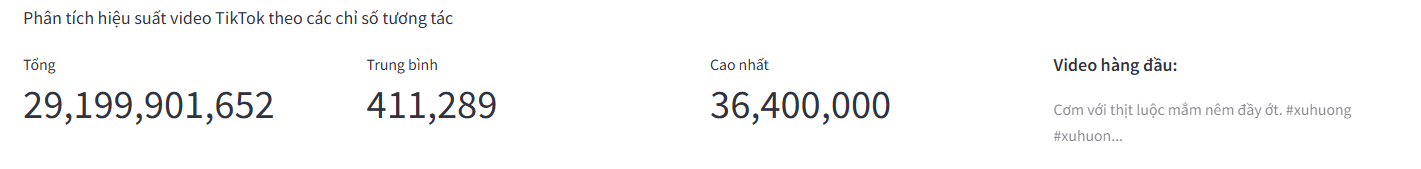
\includegraphics[width=6.5in]{img/6-4-1-A.png}}
        \caption{Thống kê tổng quan.}
    \end{figure}

    \item \textbf{Hiệu suất theo Thời lượng Video:} Biểu đồ kết hợp hiển thị số lượng video (biểu đồ cột) và chỉ số tương tác đã chọn theo kiểu tổng hợp (biểu đồ đường) cho từng khoảng thời lượng video. Thời lượng được phân loại trước theo từng bins.
    \begin{figure}[H]
        \centering
        \frame{
        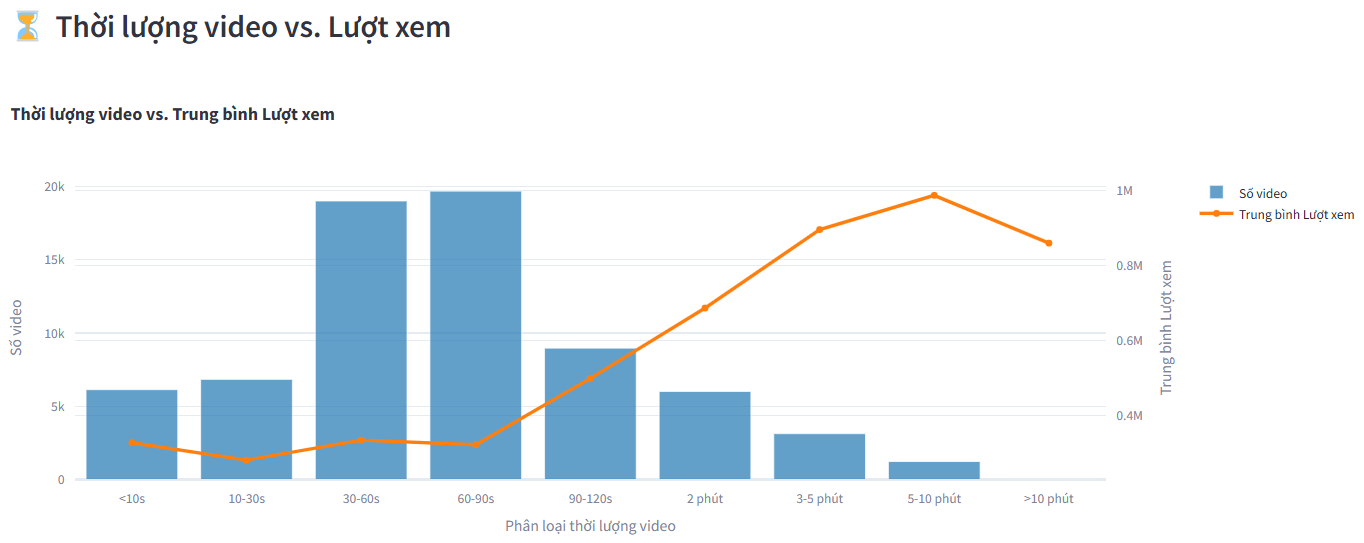
\includegraphics[width=6.5in]{img/6-4-1-B.png}}
        \caption{Thời lượng video vs. Lượt xem.}
    \end{figure}
    
    \item \textbf{Hiệu suất theo Thời gian đăng:} Biểu đồ tương tự phân tích chỉ số theo giờ đăng trong ngày (\texttt{posting\_hour} trích xuất từ \texttt{createTime.dt.hour}) và ngày đăng trong tuần (\texttt{posting\_day} trích xuất từ \texttt{createTime.dt.day\_name()}).
    \begin{figure}[H]
        \centering
        \frame{
        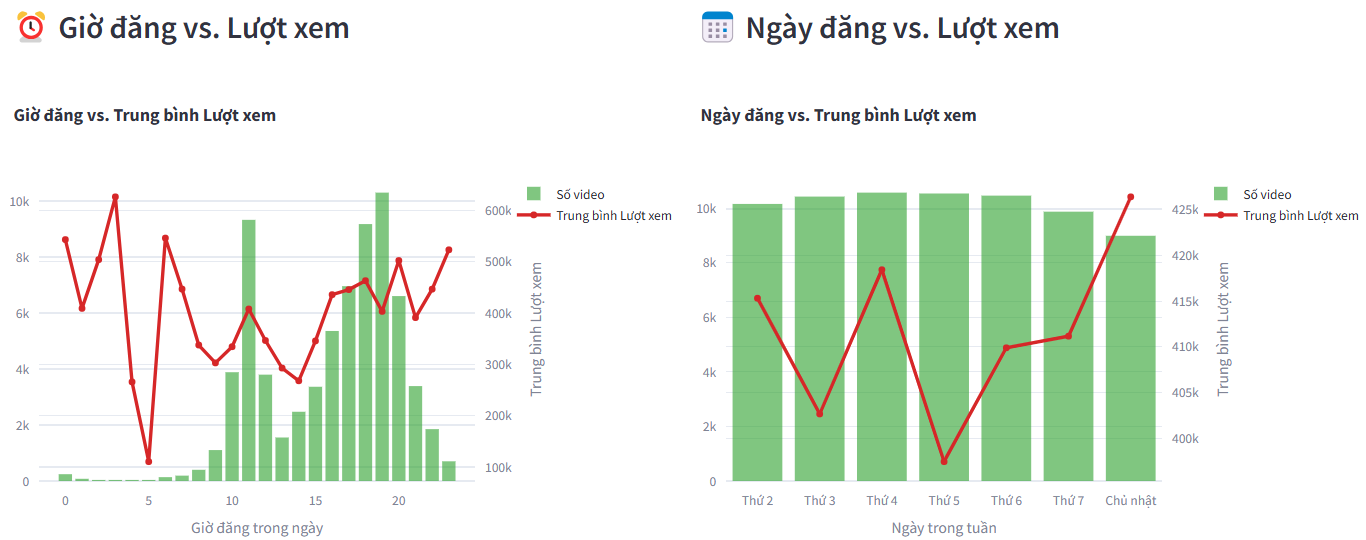
\includegraphics[width=6.5in]{img/6-4-1-C.png}}
        \caption{Thời gian đăng vs. Lượt xem.}
    \end{figure}
    
    \item \textbf{Top 5 Video theo chỉ số hiệu suất:} Hiển thị bảng (sử dụng \texttt{st.dataframe}) liệt kê 5 video có hiệu suất cao nhất dựa trên chỉ số được chọn khi lọc filter ở thanh bên.
    \begin{figure}[h]
        \centering
        \frame{
        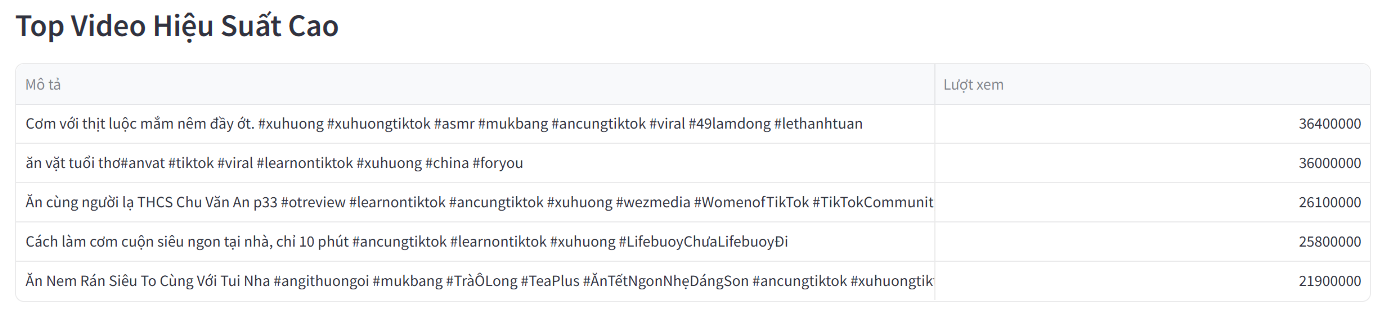
\includegraphics[width=6.5in]{img/6-4-1-D.png}}
        \caption{Top Video Hiệu Suất Cao.}
    \end{figure}
\end{itemize}

\paragraph{Tính năng bổ sung:}
    \begin{itemize}
        \item \textbf{Nhận xét AI:} Tích hợp nhận xét tự động (sử dụng Gemini API) cho các biểu đồ phân tích theo thời lượng và thời gian đăng. Các nhận xét này được tạo dựa trên dữ liệu tóm tắt (\texttt{groupby(...).agg(...).to\_string()}) của biểu đồ tương ứng.
        
        \item \textbf{Tải dữ liệu:} Nút \texttt{download\_button} cho phép người dùng tải xuống toàn bộ dữ liệu đã xử lý dưới dạng file CSV.
    \end{itemize}


\subsubsection{Phân tích Hashtag Tổng quan}

Module này cung cấp cái nhìn tổng thể về việc sử dụng và hiệu quả của các hashtag trong tập dữ liệu.

\paragraph{Mục tiêu:} Khám phá các hashtag phổ biến, hiệu quả, xu hướng sử dụng và ảnh hưởng của số lượng hashtag đến hiệu suất video.

\paragraph{Tùy chọn / Filter:} Người dùng chọn chỉ số, số lượng N (\texttt{top\_n}) cho các bảng xếp hạng, và đơn vị thời gian (Ngày/Tuần/Tháng) cho biểu đồ xu hướng.

\paragraph{Phân tích chính:}
    \begin{itemize}
        \item \textbf{Top N Hashtag hiệu quả:} Biểu đồ tính tổng chỉ số tương tác (\texttt{total\_engagement}), số lượng video (\texttt{video\_count}), và tương tác trung bình (\texttt{avg\_engagement}) cho mỗi hashtag. Biểu đồ kết hợp tổng tương tác và tương tác/video vs cho số video sử dụng trục Y phụ.
        \begin{figure}[H] % Use [H] to force fixed placement
            \centering
            \frame{
            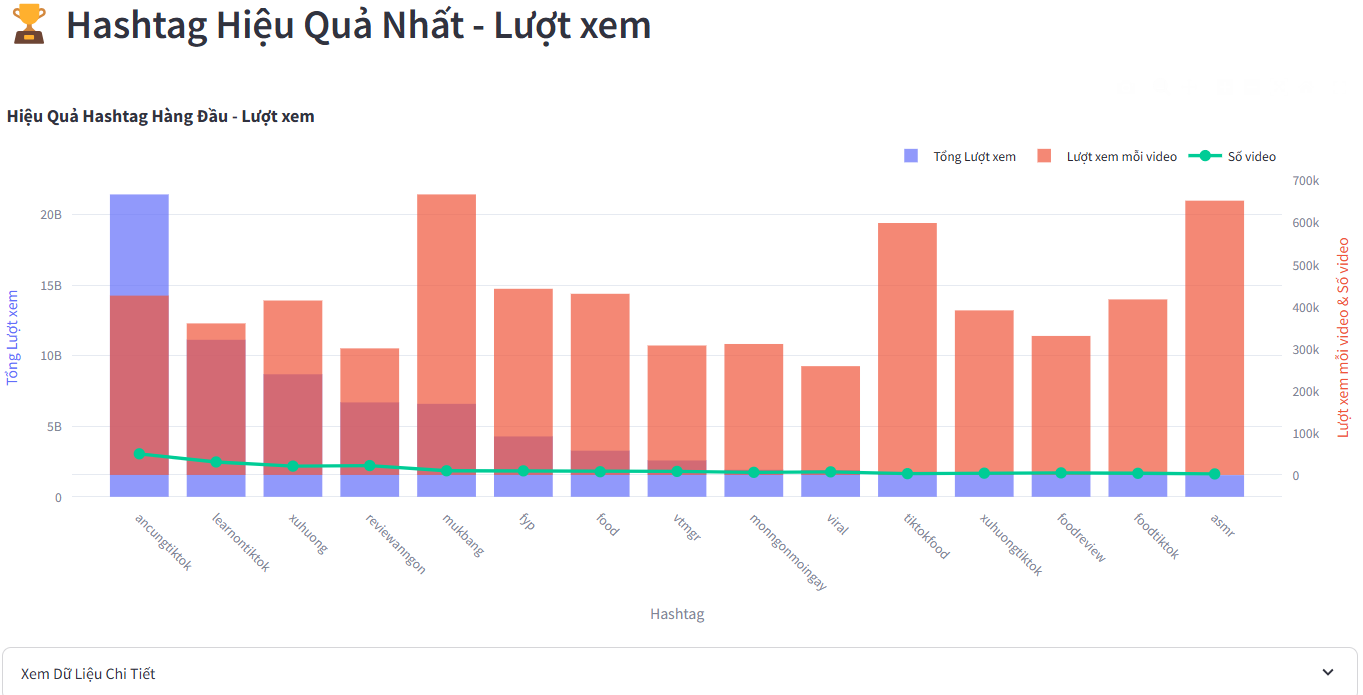
\includegraphics[width=6.5in]{img/6-4-2-A.png}}
            \caption{Hashtag Hiệu Quả Nhất.}
        \end{figure}

        \item \textbf{Số lượng Hashtag tối ưu:} Biểu đồ sử dụng nhóm dữ liệu theo \texttt{hashtag\_count} (số lượng hashtag mỗi video) và tính toán tương tác trung bình (\texttt{avg\_engagement}), số lượng video (\texttt{video\_count}), và trung vị (\texttt{median\_engagement}). Biểu đồ trực quan hóa mối quan hệ giữa số lượng hashtag và tương tác trung bình, với kích thước điểm biểu thị số lượng video và có thêm đường xu hướng.
        \begin{figure}[H]
            \centering
            \frame{
            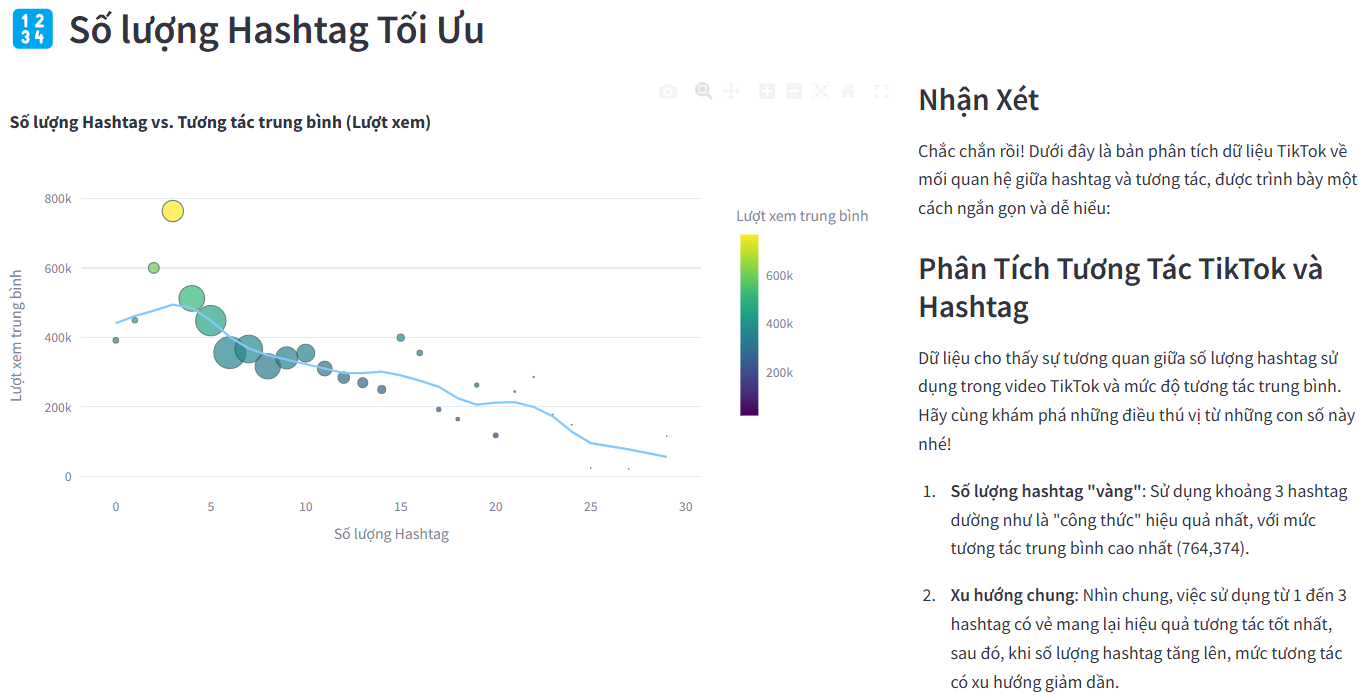
\includegraphics[width=6.5in]{img/6-4-2-B.png}}
            \caption{Số lượng Hashtag Tối Ưu.}
        \end{figure}
        
        \item \textbf{Xu hướng Hashtag theo thời gian:} Biểu đồ lọc ra top N hashtag hiệu quả nhất (dựa trên chỉ số phân tích), sau đó nhóm dữ liệu đã \texttt{explode} theo đơn vị thời gian được chọn và hashtag, rồi vẽ biểu đồ đường thể hiện tổng chỉ số tương tác theo thời gian cho từng hashtag. Có thể lựa chọn filter mốc thời gian trên biểu đồ.
        \begin{figure}[H]
            \centering
            \frame{
            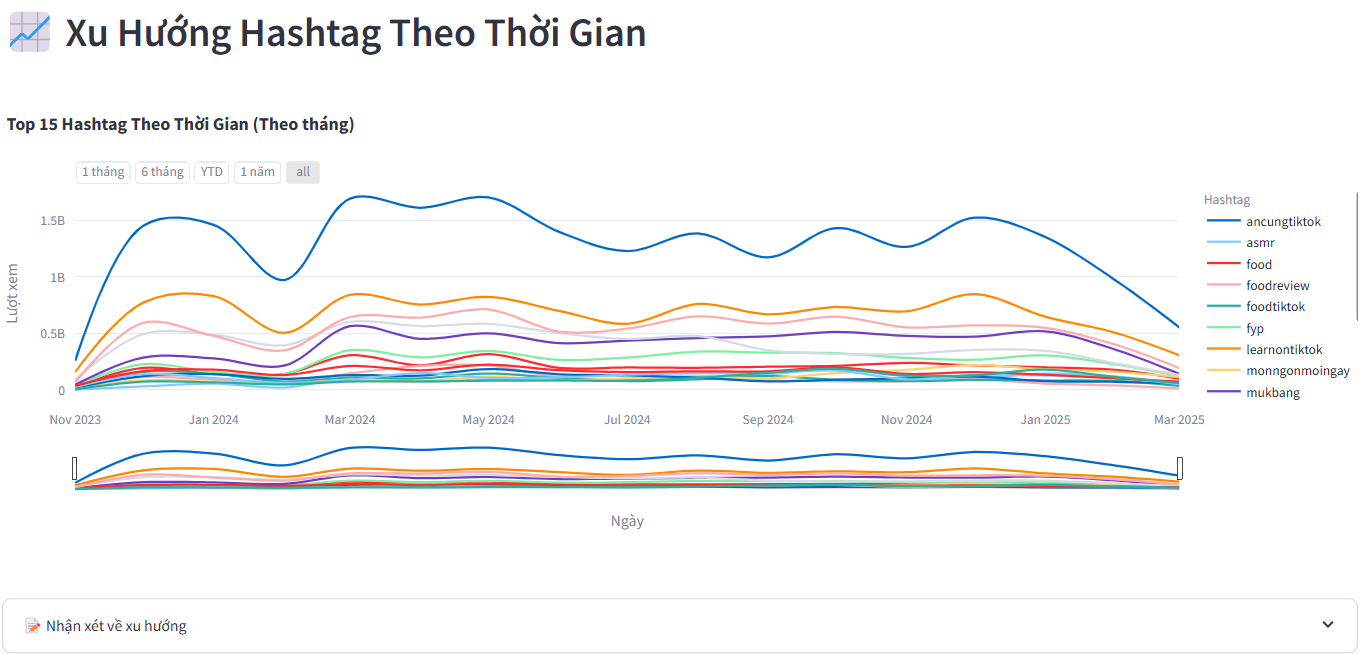
\includegraphics[width=6.5in]{img/6-4-2-C.png}}
            \caption{Xu Hướng Hashtag Theo Thời Gian.}
        \end{figure}
    \end{itemize}

\paragraph{Tính năng bổ sung:}
    \begin{itemize}
        \item \textbf{Nhận xét AI:} Tích hợp nhận xét tự động từ Gemini cho biểu đồ phân tích số lượng hashtag và biểu đồ xu hướng hashtag, hiển thị trong window expander hoặc cột riêng.
    \end{itemize}


\subsubsection{Phân tích Hashtag Đơn lẻ}

Module này cho phép người dùng đi sâu vào phân tích hiệu suất và bối cảnh sử dụng của một hashtag cụ thể.

\paragraph{Mục tiêu:} Hiểu rõ hiệu suất theo thời gian, các hashtag liên quan và những người dùng (tác giả) sử dụng hashtag đó hiệu quả nhất.

\paragraph{Tùy chọn:} Người dùng chọn hashtag cụ thể từ danh sách (danh sách drop-down được lấy từ dữ liệu), chọn chỉ số phân tích, đơn vị thời gian, và số lượng N (\texttt{top\_n} qua slide filter ở thanh bên).

\paragraph{Phân tích chính (cho hashtag được chọn):}
    \begin{itemize}
        \item \textbf{Lọc dữ liệu:} Thanh bên được sử dụng để tạo ra một filter con chỉ chứa các video có chứa hashtag được chọn (so sánh không phân biệt chữ hoa/thường). Nếu không có dữ liệu, cảnh báo (\texttt{warning}) sẽ được hiển thị.
        \begin{figure}[H]
            \centering
            \frame{
            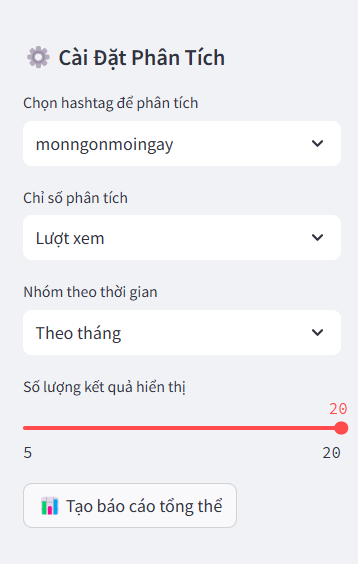
\includegraphics[width=1.5in]{img/6-4-3-Filter.png}}
            \caption{Cài đặt filter cho report}
        \end{figure}

        \item \textbf{Thống kê tổng quan:} Hiển thị tổng quan tính toán các chỉ số tổng hợp (tổng video, tổng/trung bình/trung vị tương tác) cho hashtag đã lọc và hiển thị bằng thanh metric.
        \begin{figure}[H]
            \centering
            \frame{
            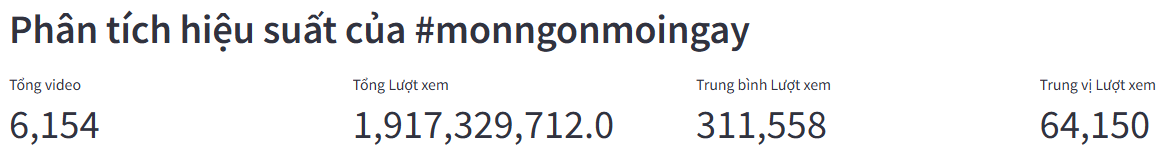
\includegraphics[width=6.5in]{img/6-4-3-A.png}}
            \caption{Phân tích hiệu suất của \#monngonmoingay.}
        \end{figure}
        
        \item \textbf{Xu hướng hiệu suất theo thời gian:} Biểu đồ nhóm dữ liệu đã lọc theo đơn vị thời gian (\texttt{time\_group}) và vẽ biểu đồ đường thể hiện tổng chỉ số tương tác theo thời gian.
        \begin{figure}[H]
            \centering
            \frame{
            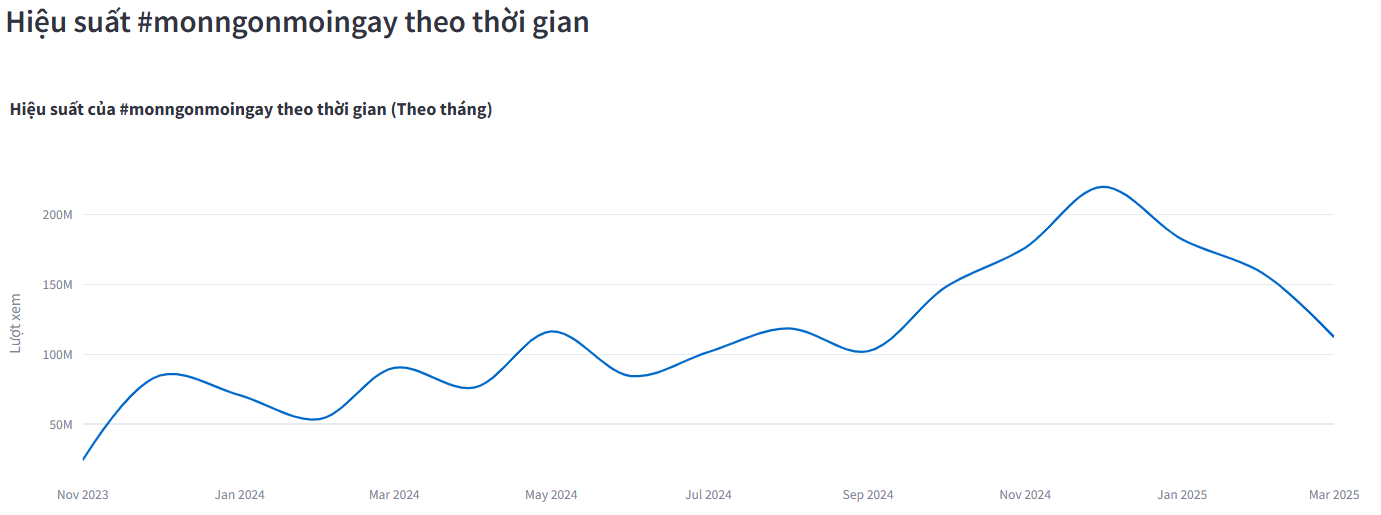
\includegraphics[width=6.5in]{img/6-4-3-B.png}}
            \caption{Hiệu suất \#monngonmoingay theo thời gian.}
        \end{figure}
        
        \item \textbf{Hashtag đồng xuất hiện (Co-occurring):} Biểu đồ hiển thị data về các video chứa hashtag mục tiêu, đầu tiên loại bỏ hashtag mục tiêu, đếm tần suất xuất hiện của các hashtag còn lại và vẽ biểu đồ cột hiển thị top N hashtag thường xuất hiện cùng nhất.
        \begin{figure}[H]
            \centering
            \frame{
            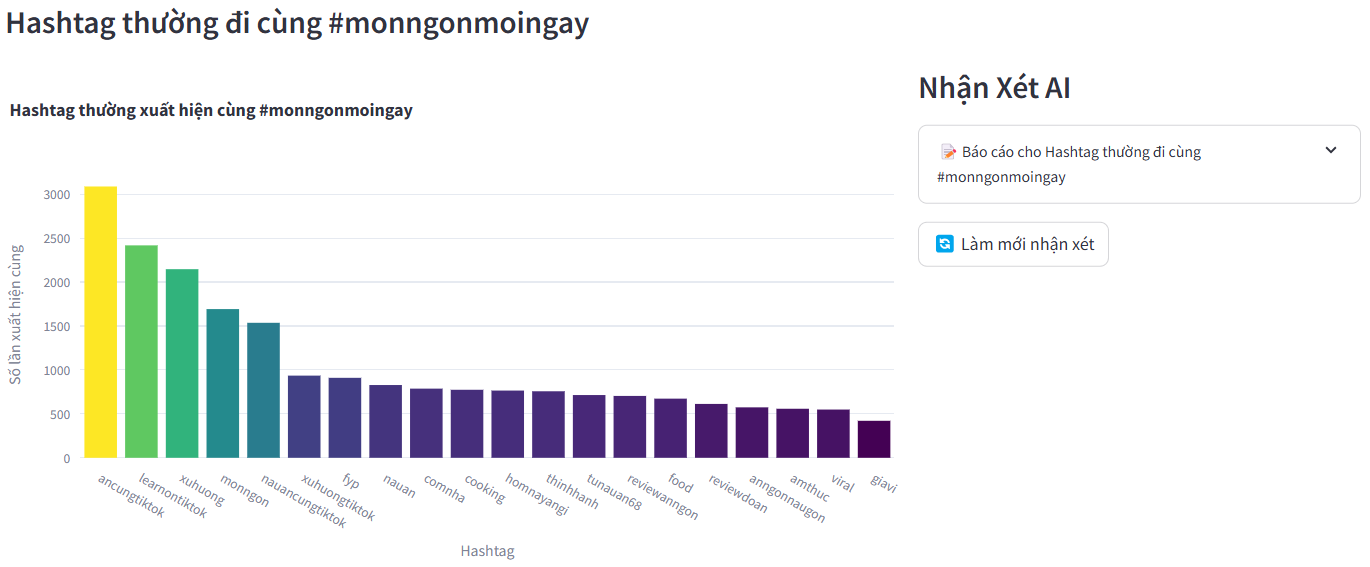
\includegraphics[width=6.5in]{img/6-4-3-C.png}}
            \caption{Hashtag thường đi cùng \#monngonmoingay.}
        \end{figure}
        
        \item \textbf{Tác giả hiệu quả nhất:} Biểu đồ sử dụng nhóm dữ liệu đã lọc theo \texttt{author.uniqueId}, tính tổng chỉ số tương tác (\texttt{total\_engagement}), số video (\texttt{video\_count}), và tương tác trung bình (\texttt{avg\_engagement}), sau đó vẽ biểu đồ cột hiển thị top N tác giả có tổng tương tác cao nhất khi sử dụng hashtag này.
        \begin{figure}[H]
            \centering
            \frame{
            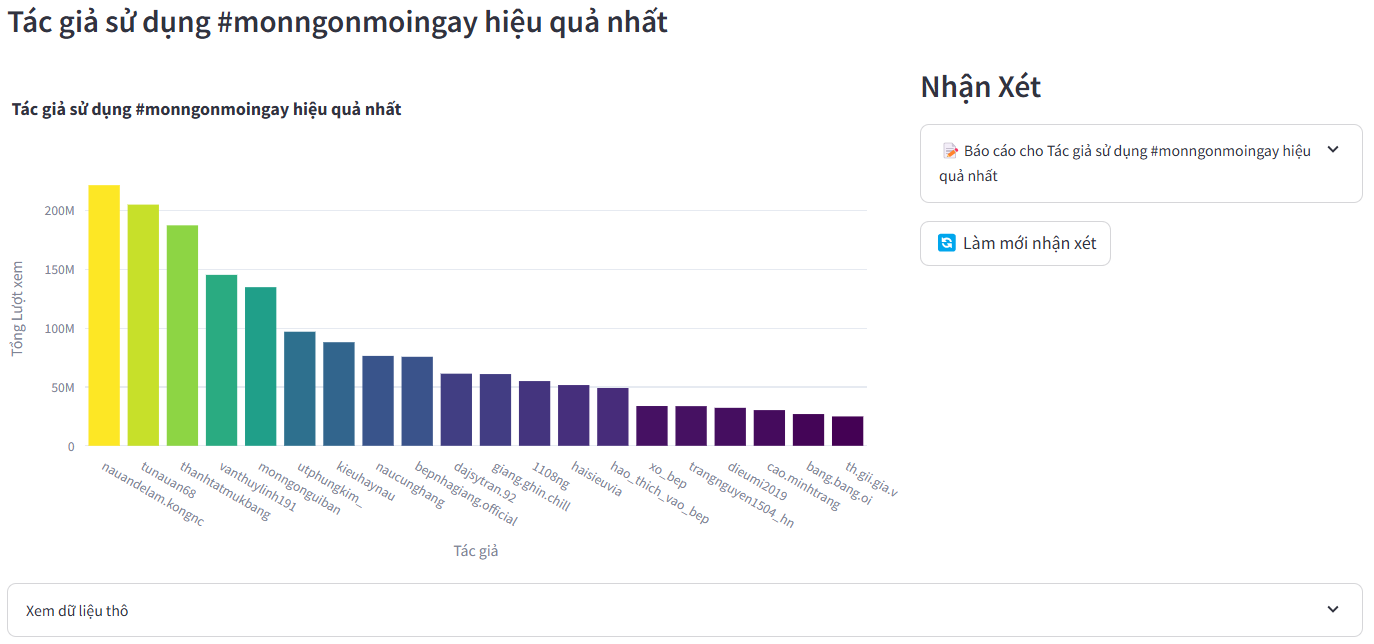
\includegraphics[width=6.5in]{img/6-4-3-D.png}}
            \caption{Tác giả sử dụng \#monngonmoingay hiệu quả nhất.}
        \end{figure}
    \end{itemize}

\paragraph{Tính năng bổ sung:}
    \begin{itemize}
        \item \textbf{Nhận xét AI:} Tích hợp nhận xét tự động từ Gemini cho phân tích hashtag đồng xuất hiện và phân tích tác giả hiệu quả, hiển thị trong window expander. Các prompt được thiết kế để yêu cầu Gemini phân tích về chủ đề liên quan, đặc điểm tác giả, khoảng cách hiệu suất, và gợi ý chiến lược.
        
        \item \textbf{Xem dữ liệu thô:} Cho phép người dùng xem bảng dữ liệu của các video chứa hashtag được chọn, sắp xếp theo chỉ số tương tác.
    \end{itemize}


\subsection{Tích hợp Trí tuệ Nhân tạo (AI)}

Một tính năng nổi bật của dashboard là việc tích hợp mô hình ngôn ngữ lớn (LLM) Google Gemini để cung cấp các nhận xét và phân tích tự động, giúp người dùng nhanh chóng nắm bắt các insight quan trọng từ dữ liệu trực quan hóa.

\begin{itemize}
    \item \textbf{Thư viện và Khởi tạo:} Sử dụng thư viện \texttt{google.genai}. Client kết nối đến API được khởi tạo và cache bằng hàm \texttt{get\_genai\_client} được đánh dấu \texttt{@st.cache\_resource} trong mỗi module phân tích.
    
    \item \textbf{Hàm Tạo Báo cáo:} Đầu tiên nhận một chuỗi dữ liệu (\texttt{data\_str}, thường là kết quả tóm tắt từ DataFrame hoặc sau khi áp dụng các bước filter / transformation và một prompt yêu cầu phân tích. Prompt được thiết kế bằng tiếng Việt, yêu cầu mô hình đóng vai trò nhà phân tích dữ liệu, đưa ra các insight ngắn gọn, dễ hiểu dưới dạng Markdown. Kết quả trả về (văn bản nhận xét) được cache tối ưu cho \texttt{streamlit}.
    
    \item \textbf{Ứng dụng trong Dashboard:} Các nhận xét AI được tạo và hiển thị bên cạnh hoặc dưới các biểu đồ chính trong mỗi trang phân tích, thường nằm trong một window expander để tiết kiệm không gian. Ví dụ: nhận xét về mối quan hệ giữa thời lượng video và tương tác, gợi ý số lượng hashtag tối ưu, phân tích xu hướng hashtag, nhận định về các hashtag liên quan hoặc đặc điểm của các tác giả hàng đầu.
\end{itemize}